\documentclass[11pt, journal]{IEEEtran}

% Packages
\usepackage{cite}
\usepackage{graphicx}
\usepackage{amsmath,amssymb,amsfonts}
\usepackage{algorithmic}
\usepackage{textcomp}
\usepackage{xcolor}
\usepackage{tikz}
\usepackage{pgf-umlcd}
\usepackage{tcolorbox}

% Title and Author
\title{SQLiteCache: A single-threaded, persistent, and high capacity key-value cache using SQLite}

\author{
    \IEEEauthorblockN{
        Christofer Washington Berruz Chungata\IEEEauthorrefmark{1},
        Mithi Pandey\IEEEauthorrefmark{2}\\
    }
    \IEEEauthorblockA{
        \textit{Department of Computer Science}, \\
        \textit{San Jos\'{e} State University}, \\
        San Jos\'{e}, California, U.S.A \\
        \IEEEauthorrefmark{1}christoferwashington.berruzchungata@sjsu.edu, \\
        \IEEEauthorrefmark{2}mithi.pandey@sjsu.edu
    }
}

\begin{document}

\maketitle

\begin{abstract}
The abstract goes here. It should summarize the key points of your paper in about 150–250 words.
\end{abstract}

\begin{IEEEkeywords}
Keyword1, Keyword2, Keyword3, Keyword4
\end{IEEEkeywords}

\newcommand{\sqlitecache}{\mbox{\tt sqlitecache\tt}}
\section{Introduction}
% Project goals and motivation
% Description of Database systems challenge addressed
The introduction goes here. Provide background, motivation, and an overview of the paper.

\section{Related Work}
% Survey related work in the related work section
Discuss related work and how your work differs or builds upon it.

\section{Methodology}
% Include a detailed description of your methodology, analysis, and implementation in the technical section
% o Describe key design goals in designing your database
% o Describe the key components and algorithms
% o Describe your architecture and how the components will interact.
%   You must include several UML diagrams to illustrate your design
%   (at least 3 diagrams from below list to illustrate proper overview of the system.
%   ▪ Use Case style diagram to show the overview of your system functionality and different functions in your system.
%   ▪ Use the Deployment and Component diagrams to show the software and hardware components of your system.
%   ▪ Communication diagram to illustrate the connections between the components,
%   ▪ Sequence diagram explains the sequence of actions, events, and processes between the components,
%       objects, and actors in your system.
%   ▪ Activity and State diagrams to explain more detail about a process or object in your system.

In this project, we designed and implemented a
persistent key-value cache using SQLite
that supports three eviction policies: Least Recently Used (LRU),
Least Frequently Used (LFU), and a hybrid policy combining both LRU and LFU
described in \cite{shah2023ImprovedCacheEviction}.


Our key design goals of this project are:
\begin{itemize}
    \item \textbf{Single-threaded}: The cache should be
        single-threaded to simplify the design and avoid concurrency issues.
    \item \textbf{Persistent}: The cache should persist data to disk using SQLite, allowing for data recovery after a crash.
    \item \textbf{High capacity}: The cache should be able to store a large amount of data efficiently.
    \item \textbf{Eviction policies}: The cache should support LRU, LFU, and a hybrid policy for eviction.
    \item \textbf{Encryption}: The cache should support encryption to protect sensitive data.
    \item \textbf{Compression}: The cache should support compression to reduce the size of the data stored on disk.
    \item \textbf{Ease of use}: The cache should be easy to use and integrate into existing applications.
    \item \textbf{Cross-platform}: The cache should work on any platform that supports SQLite.
\end{itemize}

Our persistent cache is available as a pip installable package,
\sqlitecache, that
can be used for any Python application.
The overall design of the architecture is shown in Figure \ref{fig:architecture}.

As part of this project, we also include a simulation 
comparing the hit rate
and miss rates of the three policies to determine which one performs better
in terms of cache performance. The methodology is similar to \cite{shah2023ImprovedCacheEviction},
with the major difference that our cache is disk based and persistent,
while the cache in \cite{shah2023ImprovedCacheEviction} is memory based and not persistent.
Additionally, the authors in \cite{shah2023ImprovedCacheEviction} use an element-oriented
cache while we use a key-value cache. More details on the simulation
are provided in Section \ref{sec:simulation}.

% Overall architecture
\begin{figure}[ht]
    \centering
    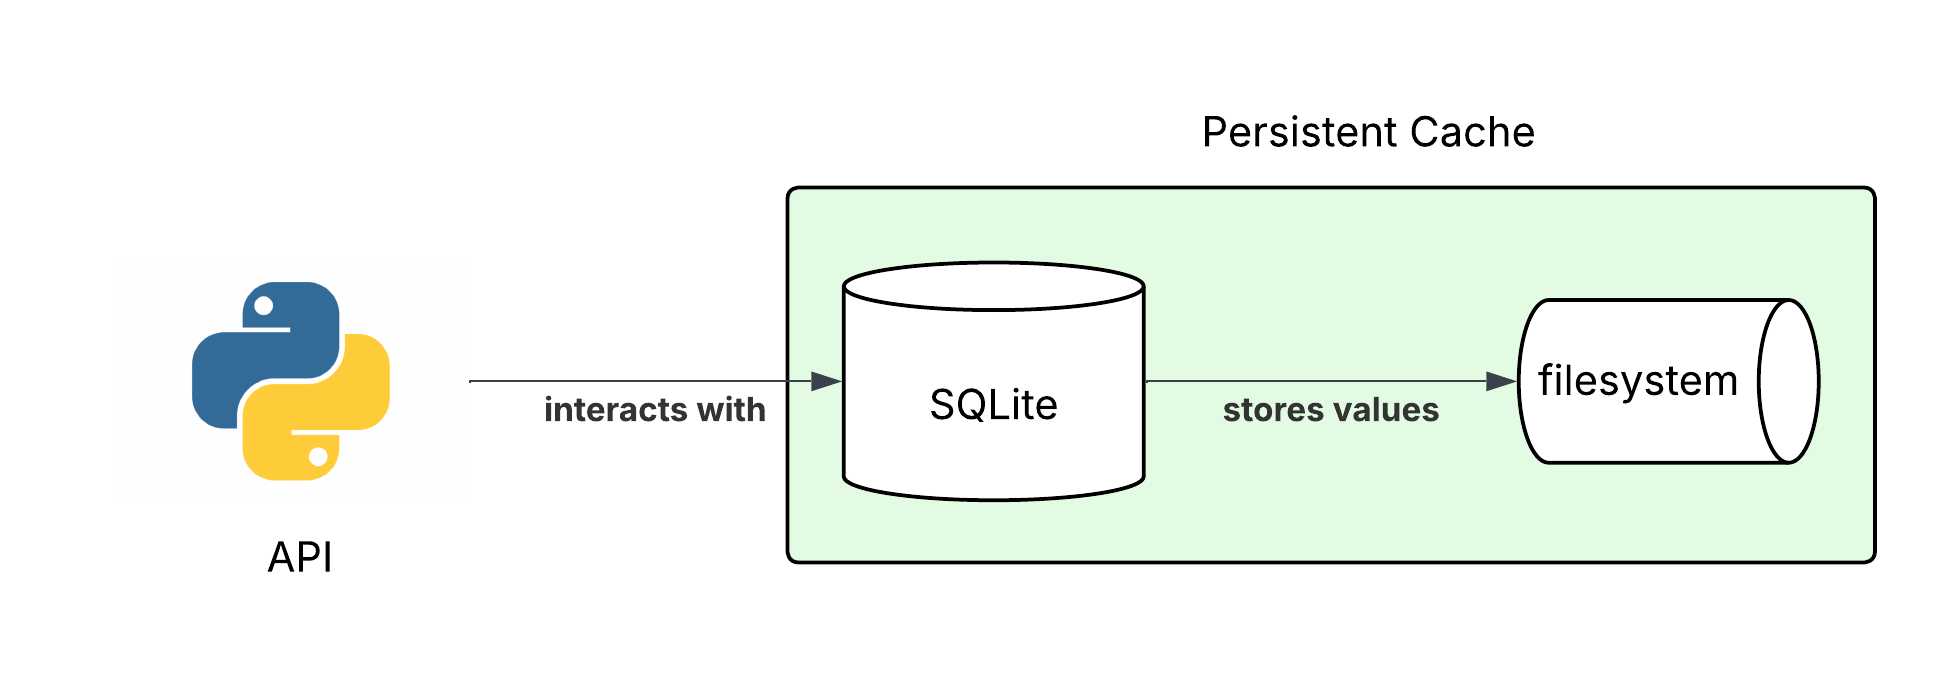
\includegraphics[width=3.25in]{images/overall_architecture.png}
    \caption{Architecture of SQLiteCache}
    \label{fig:architecture}
\end{figure}

\subsection{Key Components}
The \sqlitecache~package exposes three main cache classes: LRUCache, LFUCache, and HybridCache.
Furthermore, we use the concept of a DiskStorage that is a wrapper around the filesystem
and it is used alongside SQLite to persist data to disk, as shown in Figure \ref{fig:architecture}.

These cache classes can be divided into two groups: functional caches and wrapper caches.

Both LRUCache and LFUCache are functional caches because they store data
in a combination of relations and filesystem.
HybridCache behaves like a soft wrapper around LRUCache and LFUCache because
it uses the composition pattern to combine the two caches. At any point in time,
elements in the HybridCache are stored in either LRUCache or LFUCache, but not both.
The entire inheritance hierarchy is shown in Figure \ref{fig:base_cache_uml_diagram}
and Figure \ref{fig:real_caches_uml_diagram}.


% UML inheritance diagram of the base classes
\begin{figure}
    \centering
    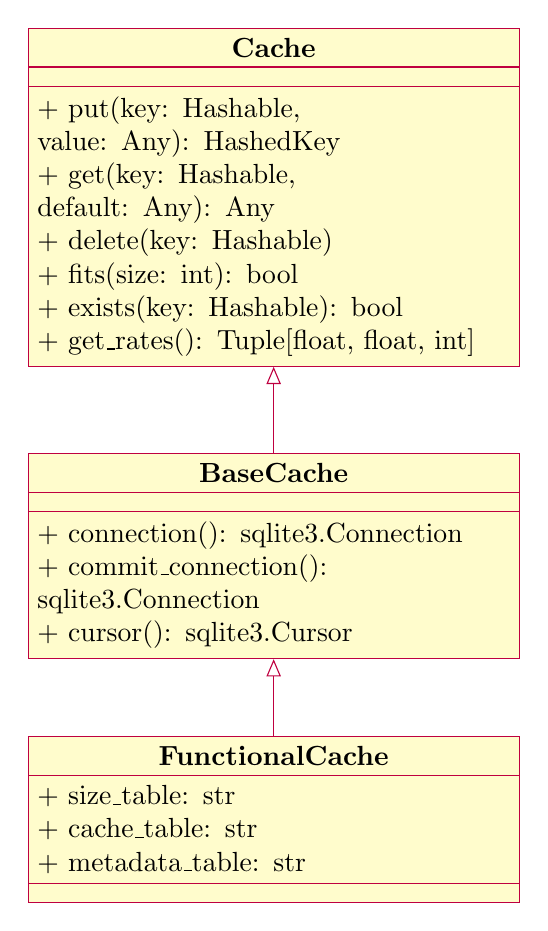
\begin{tikzpicture}[scale=0.45]
        % Base class
        \begin{class}[text width=6cm]{Cache}{0, 0}
            \operation{+ put(key: Hashable, value: Any): HashedKey}
            \operation{+ get(key: Hashable, default: Any): Any}
            \operation{+ delete(key: Hashable)}
            \operation{+ fits(size: int): bool}
            \operation{+ exists(key: Hashable): bool}
            \operation{+ get\_rates(): Tuple[float, float, int]}
        \end{class}

        % Derived classes
        \begin{class}[text width=6cm]{BaseCache}{0, -12}
            \inherit{Cache}
            \operation{+ connection(): sqlite3.Connection}
            \operation{+ commit\_connection(): sqlite3.Connection}
            \operation{+ cursor(): sqlite3.Cursor}
        \end{class}

        % FunctionalCache
        \begin{class}[text width=6cm]{FunctionalCache}{0, -20}
            \inherit{BaseCache}
            \attribute{+ size\_table: str}
            \attribute{+ cache\_table: str}
            \attribute{+ metadata\_table: str}
        \end{class}
    \end{tikzpicture}
    \caption{UML class diagram of the base cache classes.}
    \label{fig:base_cache_uml_diagram}
\end{figure}


% UML inheritance diagram of the real cache classes (LRUCache, LFUCache, HybridCache)
\begin{figure}
    \centering
    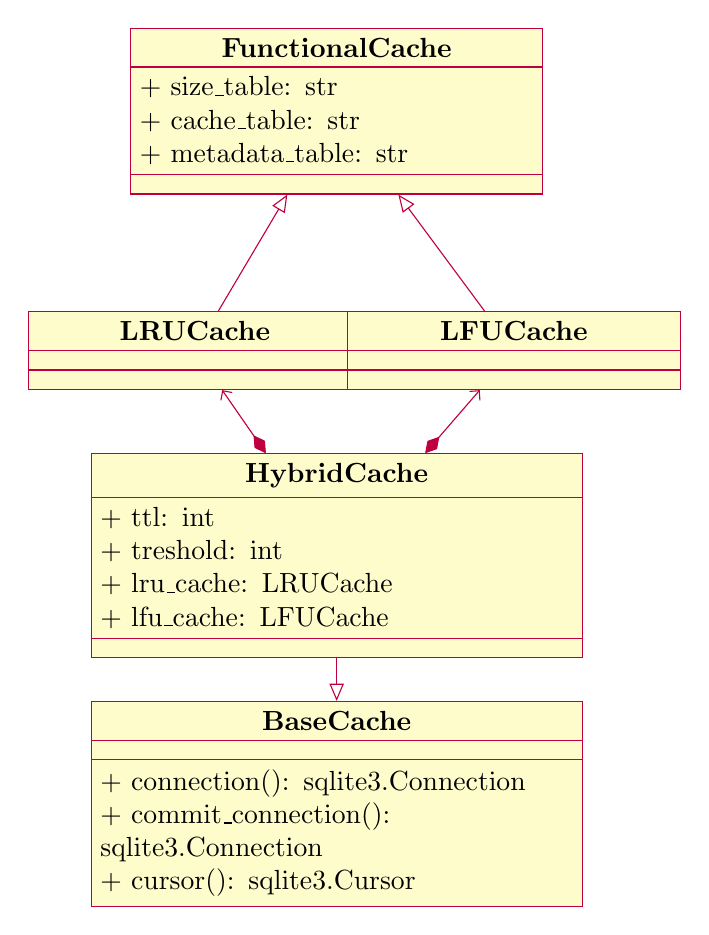
\begin{tikzpicture}[scale=0.45]
        % FunctionalCache
        \begin{class}[text width=5cm]{FunctionalCache}{0, 0}
            \attribute{+ size\_table: str}
            \attribute{+ cache\_table: str}
            \attribute{+ metadata\_table: str}
        \end{class}
        % LRUCache and LFUCache
        \begin{class}[text width=4cm]{LRUCache}{-4, -8}
            \inherit{FunctionalCache}
        \end{class}

        \begin{class}[text width=4cm]{LFUCache}{5, -8}
            \inherit{FunctionalCache}
        \end{class}

        % BaseCache
        \begin{class}[text width=6cm]{BaseCache}{0, -19}
            \operation{+ connection(): sqlite3.Connection}
            \operation{+ commit\_connection(): sqlite3.Connection}
            \operation{+ cursor(): sqlite3.Cursor}
        \end{class}

        % HybridCache
        \begin{class}[text width=6cm]{HybridCache}{0, -12}
            \inherit{BaseCache}
            \attribute{+ ttl: int}
            \attribute{+ treshold: int}
            \attribute{+ lru\_cache: LRUCache}
            \attribute{+ lfu\_cache: LFUCache}
        \end{class}
        \composition {HybridCache}{}{}{LRUCache}
        \composition {HybridCache}{}{}{LFUCache}
    \end{tikzpicture}
    \caption{UML class diagram showing the relation of the three policy caches
    and their relation to the base classes.}
    \label{fig:real_caches_uml_diagram}
\end{figure}


\subsection{LRUCache and LFUCache}
LRUCache and LFUCache use a combination of a database and the filesystem
to store data. For a given (key, value) pair submitted to the cache,
the cache computes a hash of the key. Hash collisions are handled by replacement
instead of chaining. Formally, the keys stored in the cache are $k' = hash(k)$,
where $k$ is the original key and $k'$ is the hashed key.
Our hashing function is defined as $$ hash(k) = PythonHash(k) \times \mathrm{0xFFFFFFFF}$$
As a result, the keys must implement the \texttt{\_\_hash\_\_} method.

Once $k'$ is computed, the database sends $v$ to the DiskStorage.
To store $v$, we first
compute its binary representation, $v_b$ using the \texttt{pickle} module.
By using pickle, we guarantee that any Python object
that can be serialized and deserialized using
the \texttt{pickle} module can be stored in the cache.
If compression is enabled, we compress the data using the \texttt{zlib} module.
If encryption is enabled, we encrypt the data using the \texttt{cryptography}
module. Once the final binary value $v_b'$ is obtained,
the DiskStorage object creates a unique
filename, $f_{name}$, using the \texttt{uuid} library.
Then, DiskStorage saves $v_b'$ into the filepath $dir/f_{name}$ where $dir$ is the directory
used to initialize the DiskStorage object. Finally, DiskStorage sends the full filepath
back to the database and the database stores the (key, filepath) pair in the cache table.

Note that depending on the eviction policy of the cache, extra information
is inserted into the cache table. These differences are described in
Section \ref{sec:lru} and Section \ref{sec:lfu}.

The functionality between LRUCache and LFUCache
is similar, creating the inheritance relationship described in Figure \ref{fig:real_caches_uml_diagram}.
Furthermore, one design choice is that each cache class has its own cache table,
metadata table, and size table. This is achieved by each relation having a suffix
that is the name of the cache class. As a result, it is possible to have
one cache of each type in the same SQLite database. This is extremely useful
for testing and debugging the HybridCache class,
which uses one LRUCache and one LFUCache
as its backing caches.

\begin{tcolorbox}[colback=blue!5!white, colframe=blue!75!black, title=Note]
    To avoid confusion and complexity, it is recommended to use
    one cache instance per SQLite database.
\end{tcolorbox}

% create a note using the 
\subsection{LRUCache\label{sec:lru}}
\subsection{LFUCache\label{sec:lfu}}

\subsection{DiskStorage}

\subsection{Simulation\label{sec:simulation}}

\section{Results and Discussion}
% Describe evaluation methodology and significant results in the evaluation section
% Evaluate the selected approach and analyze why the selected approach is good?
%   Provide an intuitive description of the algorithms, their correctness and their complexity
Present your results and discuss their implications.

\section{Conclusion}
% Conclusions, lessons learned possible improvements, etc.
Summarize your findings and suggest future work.

\bibliographystyle{IEEEtran}
\bibliography{references}

\end{document}